% !TEX program = xelatex
% [EN] Reuse the Chinese edition's source images and citation keys. / [CN] 复用中文版的原始资料图与文献标识。
\documentclass[11pt,a4paper]{article}
\usepackage[margin=24mm]{geometry}
\usepackage{fontspec}
\setmainfont{TeX Gyre Termes}
\setsansfont{TeX Gyre Heros}
\usepackage{amsmath,booktabs,tabularx,array,longtable}
\usepackage{graphicx,caption,xurl}
\usepackage[hidelinks]{hyperref}
\graphicspath{{figures/beam-intensity-sources/}}
\captionsetup{font=small,labelfont=bf,hypcap=false}
\hypersetup{pdftitle={Beam Intensity from PIS to SRC and ATT Control},pdfauthor={DPOLAR project}}
\setlength{\parindent}{0pt}
\setlength{\parskip}{5pt}
\setlength{\emergencystretch}{2em}
\renewcommand{\arraystretch}{1.15}
\widowpenalty=10000
\clubpenalty=10000
\newcolumntype{Y}{>{\raggedright\arraybackslash}X}
\title{Beam Intensity from PIS to SRC\\and ATT Control\\[4pt]\large Connection to BigRIPS F2/F3 downstream of SRC}
\author{DPOLAR beamline notes}
\date{English edition, 8 September 2026}
\begin{document}
\maketitle

\begin{abstract}
Polarized deuterons are accelerated through PIS--AVF--RRC--SRC. The source output of $<100\,\mu\mathrm{A}$, the $10\,\mathrm{nA}$ used in a recovery test downstream of AVF, and the expected SRC intensity of $30\,\mathrm{pnA}$ at $250\,\mathrm{MeV/u}$ describe different quantities: source output, an experimental beam setting, and a proposal-planning value. Their ratios do not measure transmission in a single run. Beam attenuators (ATTs) reduce particle rates by combining upstream meshes; installations are documented along the AVF-to-RRC injection line. This note aligns the intensity conventions, explains ATT locations, ratios and calibration, and connects them to the downstream BigRIPS limits.
\end{abstract}

\section{Reading the intensities from PIS to SRC}
\label{sec:pis-src}
The light-ion route for polarized deuterons is
\[
\mathrm{PIS}\to\mathrm{Wien\ filter}\to\mathrm{AVF}
\to\boxed{\text{injection line with ATTs}}\to\mathrm{RRC}\to\mathrm{SRC}.
\]
This route bypasses fRC and IRC. Table~2 of the 2016 operating summary gives the following three sets of extraction energies. Each column represents one acceleration setting; all energies are in $\mathrm{MeV/u}$.\cite{sakamoto2016}
\begin{center}
\begin{tabular}{lrrr}
\toprule
Cyclotron exit & Nominal 190 & Nominal 250 & Nominal 300 \\
\midrule
AVF & 4.0 & 4.9 & 5.5 \\
RRC & 70.4 & 89.9 & 102.5 \\
SRC & 187.5 & 252.3 & 298.5 \\
\bottomrule
\end{tabular}
\end{center}

\clearpage
\textbf{The intensity table follows beamline order, but its rows refer to different years or operating conditions.} In particular, the RRC beam-service entry at $135\,\mathrm{MeV/u}$ is a different setting from the SRC injection energies above.
\begingroup
\small
\setlength{\tabcolsep}{4pt}
\begin{longtable}{@{}>{\raggedright\arraybackslash}p{0.18\linewidth}>{\raggedright\arraybackslash}p{0.13\linewidth}>{\raggedright\arraybackslash}p{0.23\linewidth}>{\raggedright\arraybackslash}p{0.39\linewidth}@{}}
\toprule
Location / report & Energy & Reported current; converted particle rate & Meaning and source \\
\midrule
\endhead
PIS ionizer exit, 2016 summary & Low-energy source beam & $<100\,\mu\mathrm{A}$; $<6.24\times10^{14}$/s & ECR ionizer output, not SRC delivery; PDF p.~2 / printed p.~146.\cite{sakamoto2016}\\
Polarimeter after AVF, 2025 report & $7\,\mathrm{MeV/u}$ & Typical $10\,\mathrm{nA}$; $6.24\times10^{10}$/s & Beam on target for the recovery test, not maximum AVF capability; INPC abstract, p.~1.\cite{sugahara2025}\\
Official RRC beam table & $135\,\mathrm{MeV/u}$ & $30\,\mathrm{pnA}$; $1.87\times10^{11}$/s & $d(\mathrm{pol.})$, AVF injection, PIS. The table is approximately 70\% of actual maxima and carries a source-development footnote.\cite{accelerator-intensity}\\
Official SRC beam table & $250\,\mathrm{MeV/u}$ & Expected $30\,\mathrm{pnA}$; $1.87\times10^{11}$/s & Proposal-planning value for $d(\mathrm{pol.})$; the source-development footnote remains.\cite{accelerator-intensity}\\
Official SRC historical maximum & $250\,\mathrm{MeV/u}$ & Instantaneous maximum $120\,\mathrm{pnA}$; $7.49\times10^{11}$/s & Maximum column of the same table; not a sustained-delivery commitment.\cite{accelerator-intensity}\\
BigDpol after SRC, 2017 paper & $186.6\,\mathrm{MeV/u}$ & $4$--$8\,\mathrm{nA}$; $(2.50$--$4.99)\times10^{10}$/s & Experimental beam on the CH$_2$ target; Sec.~II, manuscript p.~2 / PDF p.~3 including the cover.\cite{sekiguchi2017}\\
\bottomrule
\end{longtable}
\endgroup

Particle rates are calculated below, interpreting $\mu\mathrm{A}$ and $\mathrm{nA}$ for singly charged $d^+$. The official tables were checked on 8 September 2026. Their separate unpolarized-$d$ entry at $250\,\mathrm{MeV/u}$ lists $200\,\mathrm{pnA}$ expected and $1000\,\mathrm{pnA}$ instantaneous maximum; these cannot replace the polarized-beam values.\cite{accelerator-intensity} Early PIS development results and recovery history are collected in the source-status notes. The table above focuses on source output, accelerator tables and experimental beam settings.

\subsection{Units and averaging intervals}
For charge state $q$, particle rate $\dot N$, and electrical-current magnitude $I_e$,
\[
I_e=q e\dot N,\qquad I_p=e\dot N=I_e/q,
\qquad e=1.602176634\times10^{-19}\,\mathrm C.
\]
The prefix p in $\mathrm{pnA}$ denotes particle current; $\mathrm{enA}$ denotes electrical current. For $d^+$, $q=1$, so their numerical values coincide:
\[
1\,\mathrm{pnA}=6.2415\times10^9\ \text{particles/s},\qquad
10^7\ \text{particles/s}=1.602\,\mathrm{ppA}=0.001602\,\mathrm{pnA}.
\]
These are total particle rates. The area-averaged flux density is $\bar\phi=\dot N/\mathcal A$, in $\mathrm{cm^{-2}s^{-1}}$; a nonuniform beam also requires its spatial distribution. Counts per second in a scattering detector are related to incident particles per second through target thickness, cross section, acceptance and detection efficiency.

\section{What an ATT does and where it is installed}
\label{sec:att}
\textbf{A beam attenuator intercepts part of the beam with a mesh to change the particle rate.} Page~8 of the 2023 E5A visitor guide states that accelerator operators adjust the intensity by changing the combination of upstream meshes.\cite{e5a} A RILAC hardware paper describes a tantalum mesh, an insertion rod and remote on/off control. That material specification applies to the RILAC devices discussed there; it does not establish the material of every C/S-station mesh.\cite{att-hardware}

Particles passing through open mesh apertures without hitting a wire do not lose energy by traversing the mesh material. A setting $T=1/10$ means a nominal particle transmission of about 10\%, not an energy reduction to one tenth. A degrader lowers energy by passing particles through material. Scattering at wire edges can still alter the halo and accepted phase space. Nominal ATT ratios therefore do not establish the measured end-to-end transmission or, by themselves, polarization preservation.

\subsection{AVF--RRC locations and the source of ATT ratios}
The 2014 progress report explicitly lists beam-attenuation meshes in the C22, S31a and S64 diagnostic chambers. C22 is just upstream of the wall between the AVF and RRC vaults; S31a is upstream of the S3 rebuncher; S64 is downstream of the S6 rebuncher and before RRC injection. Figure~\ref{fig:att-location} reproduces the report.\cite{att-chambers}

The ratios and mesh counts below come directly from the lower-left table on page~8 of the RIKEN E5A visitor guide (2 April 2023, Rev.~1.0). At Duty $=100\%$, the page lists five mesh transmission ratios and states that operators combine upstream meshes to adjust the beam from Full to $10^{-9}$.\cite{e5a}
\begin{center}
\begin{tabular}{lrr}
\toprule
Nominal transmission $T_i$ & Transmitted fraction & Number of meshes \\
\midrule
$1/100$ & 1\% & 2 \\
$1/10$ & 10\% & 4 \\
$1/5$ & 20\% & 1 \\
$1/3$ & $\simeq33.3\%$ & 1 \\
$1/2$ & 50\% & 3 \\
\bottomrule
\end{tabular}
\end{center}
The original page is shown in Fig.~\ref{fig:e5a-att}. It lists ratios and quantities for the irradiation service, without station identifiers. The C22, S31a and S64 locations instead come from the 2014 report.\cite{att-chambers} Thus, ``ATTs upstream of SRC'' includes devices far upstream in the low-energy region; the ratio table alone cannot assign all meshes to the PIS route.

\subsection{Mesh combinations, duty factor and calibration}
As a calculation example, select two $1/2$ meshes and one each of $1/10$, $1/5$ and $1/100$. Their ideal transmission product is
\[
T_{\mathrm{example,nom}}=\frac12\frac12\frac1{10}\frac15\frac1{100}
=\frac1{20000}=5\times10^{-5}.
\]
This example specifies ratios, not installation stations. Multiplying every mesh in the irradiation-service inventory gives $8.33\times10^{-11}$. That formal product is not an operating range; the source page does not explain its difference from the stated $10^{-9}$ lower limit.

An intensity budget must specify the input measurement plane and ATT state:
\[
\langle\dot N_{\rm out}\rangle
=\dot N_{\rm in,on}\,D\,T_{\rm ATT,eff}\,\eta_{\rm rest},
\qquad T_{\rm ATT,nom}=\prod_{i\,\mathrm{IN}}T_i.
\]
Here $D$ is the beam-on fraction in the defined time window, $T_{\rm ATT,eff}$ is the effective transmission, and $\eta_{\rm rest}$ includes the remaining transport, capture and extraction efficiencies. The product approximation requires beam illumination and downstream acceptance compatible with this factorization. Do not apply $D$ again to an already averaged input, or reapply a mesh ratio to an output current already measured with that mesh inserted. Duty $=100\%$ in the E5A table does not imply an absence of RF bunches; detector pile-up still depends on the bunch structure.

Calibration uses the downstream monitor response. The 2017 Kr-beam Att scan on E5A page~8 connects low-rate plastic-scintillator counts to high-rate ionization-chamber current in their proportional region:
\[
R_{\rm PL}[\mathrm{cps}]=7.505\times10^{12}I_{\rm IC1}[\mathrm A].
\]
An aperture area of $19.63\,\mathrm{cm^2}$ converts the particle rate to average flux density (Fig.~\ref{fig:e5a-att}).\cite{e5a} The coefficient depends on the Kr beam, gas and detector configuration and cannot be transferred to deuterons. IC1 measures ionization in the gas; applying the Faraday-cup formula $I/(qe)$ directly to its current would not give the incident particle rate.

\section{Estimating ATT requirements from SRC intensity}
\label{sec:att-budget}
Suppose the SRC exit current measured with \textbf{all five meshes in the example withdrawn} is $30\,\mathrm{pnA}$, and all other transmission conditions remain unchanged after insertion. Then
\[
\dot N_{\rm SRC,0}=1.872\times10^{11}/\mathrm s,
\qquad
\dot N_{\rm SRC,ATT}\simeq\dot N_{\rm SRC,0}/20000
=9.36\times10^6/\mathrm s.
\]
Reducing that reference rate to $10^7$/s requires $T_{\rm eff}\leq5.34\times10^{-5}$, or an attenuation factor of at least $1.87\times10^4$. Starting instead from $120\,\mathrm{pnA}$ gives $3.74\times10^7$/s with the same mesh product, still above the target.

This is a conditional calculation. The official $30\,\mathrm{pnA}$ planning value does not specify the corresponding ATT combination and state, so it does not establish that inserting five meshes meets this experiment's limit. Likewise, dividing the source output of $<100\,\mu\mathrm A$ by the SRC planning value of $30\,\mathrm{pnA}$ does not measure PIS-to-SRC transmission: the values refer to different conditions.

For the after-SRC polarimeter, use the intensity measured at that location for a specified source mode, ATT combination and averaging interval. Upstream attenuation reduces the rate entering RRC/SRC and hence the rate available after SRC. A scheme that retains a higher rate after SRC and attenuates farther downstream must satisfy the acceptance and interlock conditions below.

\section{Downstream beamline layout and functions}
The first BigRIPS stage extends from the production target F0 to F2; the second extends from F3 to F7. A matching section of about 8.8~m connects F2 and F3. The stage definitions come from the official configuration page and the length from the technical table.\cite{bigrips-config,bigrips-technical}
\[
\mathrm{SRC}\to\mathrm{T\ course}\to F0\to D1/F1\to F2\to dF2\to F3.
\]
A high-power dump in the D1 gap downstream of F0 stops unreacted primary heavy ions. F1 is a momentum-dispersive focus, F2 an achromatic focus, and F3 the start of the second stage.\cite{bigrips-config} See Fig.~\ref{fig:config-source} for the source text and Fig.~\ref{fig:slit-source} for the dF2 location.

\section{Locations where the intensity can be reduced}
\begingroup\small
\noindent\begin{tabularx}{\linewidth}{@{}>{\raggedright\arraybackslash}p{0.17\linewidth}>{\raggedright\arraybackslash}p{0.26\linewidth}Y@{}}
\toprule
Location & Device & Effect on the beam \\
\midrule
Upstream RIBF accelerator region & Beam attenuator (ATT) & Mesh combinations reduce primary-beam intensity; the beam interlock system (BIS) monitors insertion states.\cite{bis}\\
After F0, inside D1 & High-power beam dump & Stops unreacted primary beam and handles beam power and shielding; not a fine, continuously variable attenuator.\cite{bigrips-config}\\
F1 & Horizontal slit, Joker slit, degrader, beam stopper & Rejects momentum tails, contaminants and halo at a dispersive plane; narrowing slits can reduce transmission.\cite{bigrips-config,bigrips-focal}\\
F2 & H/V slits, collimator, beam stopper & Restricts transverse phase space and contamination. The public configuration lists H/V slits and a 45-mm Cu stopper.\cite{bigrips-focal}\\
dF2 (F2--F3) & H/V angular-selection slits & At the point-to-parallel position, angles at F2 map to positions. Narrowing the apertures can reduce the rate reaching F3.\cite{f2-f3-slit}\\
\bottomrule
\end{tabularx}
\endgroup
The device inventories and angular-selection principle appear in Figs.~\ref{fig:focal-source} and \ref{fig:slit-source}. Reduced transmission with smaller acceptance is a beam-optics inference; the reduction depends on the incident phase-space distribution.

\section{The intensity limit at F3}
The official BigRIPS instructions require ``Total Beam Rates @ F3'' in the proposal and state a limit of $10^7$/s under radiation regulations. They recommend checking the value with Faraday Cup~2 inserted after F3 in LISE++.\cite{bigrips-intensity} Figure~\ref{fig:f3-source} reproduces the instruction. The total includes contaminants as well as the isotope of interest.

That webpage addresses RI-beam yield estimates and proposals. The 2015 BIS paper also explicitly discusses direct primary-beam delivery to instruments downstream of BigRIPS and gives a $10^7$-pps limit.\cite{bis2015} This provides primary-beam operating context for the rate scale; the area, mode and configured threshold for the proposed polarized-deuteron experiment still require beamline-team confirmation. For modes subject to the limit, trigger prescaling reduces recorded events but not the number of particles crossing F3, so it cannot replace control of the total beam rate.

\section{Primary-beam and RI-beam modes}
In standard RI production at F0, the target, D1 dump, F1 degrader/slits and F2 collimator together stop the primary beam and select RI products.\cite{bigrips-config,bigrips-focal} For primary-beam transport through BigRIPS, the 2025 BIS report states that ATT insertion states determine whether attenuation is sufficient; insufficient attenuation causes insertion of the Faraday cup at the SRC exit (Fig.~\ref{fig:bis-source}).\cite{bis}

The 2015 paper describes the earlier implementation more specifically. Frequently measured source intensity and low-energy ATT states estimate the maximum possible beam rate. FC\_G01 at the SRC exit may be withdrawn only when attenuation satisfies the condition. If an ATT state changes during operation and attenuation becomes insufficient, the beam chopper and FC\_G01 stop the beam.\cite{bis2015} This is an upper-bound estimate and protection function, not continuous non-destructive measurement of the SRC exit current. The 2025 report describes modifications to this function, so the 2015 implementation is not a complete specification of the present sequence.

The engineering implication is that a scheme retaining high intensity after SRC and reducing it only at F2 or dF2 cannot be approved from slit geometry alone. It requires confirmation of the mode-specific interlock thresholds, loss locations, slit heat loads and shielding conditions.

\section{Implications for an after-SRC polarimeter}
The following is experimental-planning advice, not an approved RIKEN operating scheme. Specify two quantities separately:
\begin{enumerate}
\item Primary-beam intensity and acceptable detector counting rates at the after-SRC polarimeter.
\item Total particle rate at F3, including contaminants, if the beam continues through BigRIPS.
\end{enumerate}
Ask the beamline team about dedicated local attenuation or an acceptable F2/dF2 collimation scheme. Ordinary F2 slits should not be assumed to be high-power beam attenuators. Where polarization must be retained, material interceptors also require evaluation of multiple scattering, energy loss, nuclear reactions and possible spin-dependent systematic effects.

\begin{thebibliography}{99}
\bibitem{sakamoto2016} N. Sakamoto et al., ``Acceleration of Polarized Deuteron Beams with RIBF Cyclotrons'', Cyclotrons 2016, TUB04, pp. 145--148, PDF p. 2 / Table 2,\newline
\url{https://proceedings.jacow.org/cyclotrons2016/papers/tub04.pdf}.
\bibitem{sugahara2025} H. Sugahara et al., ``Measurement of the polarization of the deuteron beam at RIKEN RIBF'', INPC 2025, Contribution 133, poster abstract, PDF p. 1,\newline
\url{https://indico.ibs.re.kr/event/701/contributions/6590/contribution.pdf}.
\bibitem{accelerator-intensity} RIKEN, ``Technical Information -- Beam intensity'', SRC / RRC tables and footnotes, accessed 2026-09-08,\newline
\url{https://www.nishina.riken.jp/RIBF/accelerator/tecinfo.html}.
\bibitem{sekiguchi2017} K. Sekiguchi et al., Phys. Rev. C 96, 064001 (2017), Sec. II, manuscript p. 2,\newline
\url{https://link.aps.org/accepted/10.1103/PhysRevC.96.064001}.
\bibitem{e5a} RIKEN industrial application team, E5A visitor guide, 2023-04-02, Rev. 1.0, p. 8,\newline
\href{https://ribf.riken.jp/sisetu-kyoyo/HIbeam/doc/E5Aadv_\%E8\%A6\%8B\%E5\%AD\%A6\%E6\%A1\%88\%E5\%86\%85\%E7\%94\%A8\%E8\%B3\%87\%E6\%96\%99.pdf}{RIKEN official PDF: E5A visitor guide}.
\bibitem{att-hardware} A. Uchiyama et al., ``Implementation of PIC-based Embedded I/O Controller with EPICS for RILAC Control System'', ICALEPCS 2009, WEP037, pp. 478--479, Beam Attenuators Control,\newline
\url{https://proceedings.jacow.org/icalepcs2009/papers/wep037.pdf}.
\bibitem{att-chambers} K. Yamada et al., ``Modification of beam diagnosis chambers in RILAC2 high-energy beam transport'', RIKEN Accel. Prog. Rep. 47 (2014), p. 156, Figs. 1--2 and station descriptions,\newline
\url{https://www.nishina.riken.jp/researcher/APR/APR047/pdf/156.pdf}.
\bibitem{bis2015} M. Komiyama et al., ``Recent Updates on the RIKEN RI Beam Factory Control System'', HIAT 2015, MOPA27, PDF p. 2, Upgrade of Beam Interlock System,\newline
\url{https://www.nishina.riken.jp/hiat2015/proceedings/papers/mopa27.pdf}.

\bibitem{bigrips-config} RIKEN Nishina Center, ``BigRIPS Configuration'',\newline
\url{https://www.nishina.riken.jp/ribf/BigRIPS/config.html}.
\bibitem{bigrips-technical} BigRIPS Team, ``Technical Information of BigRIPS, ZeroDegree, SAMURAI Beam Line, and OEDO Beamline'', Configuration / Length,\newline
\url{https://ribf.riken.jp/BigRIPSInfo/}.
\bibitem{bigrips-intensity} RIKEN Nishina Center, ``Secondary beam intensity expected'',\newline
\url{https://www.nishina.riken.jp/ribf/BigRIPS/intensity.html}.
\bibitem{bigrips-focal} BigRIPS Team, ``F1/F2 Chamber: standard configuration'',\newline
\url{https://ribf.riken.jp/BigRIPSInfo/chamber/f1.html},\newline
\url{https://ribf.riken.jp/BigRIPSInfo/chamber/f2.html}.
\bibitem{f2-f3-slit} K. Yoshida et al., ``Slit system between the foci F2 and F3 of the BigRIPS separator'', RIKEN Accel. Prog. Rep. 52 (2019), p. 130,\newline
\url{https://www.nishina.riken.jp/researcher/APR/APR052/pdf/130.pdf}.
\bibitem{bis} M. Komiyama et al., ``Development of a machine protection beam interlock system for the RIBF'', RIKEN Accel. Prog. Rep. 58 (2025), pp. 98--99,\newline
DOI: \href{https://doi.org/10.34448/RIKEN.APR.58-146}{10.34448/RIKEN.APR.58-146},\newline
\url{https://www.nishina.riken.jp/researcher/APR/APR058/pdf/98.pdf}.
\end{thebibliography}

The supplied \href{https://chatgpt.com/share/6a9fa6fc-7c6c-83ee-949f-a9614eb676f1}{shared discussion} and E5A PDF provided the research leads. Physical claims are supported by the original sources above; the discussion is not a measurement record of intensity or operating state.

\clearpage
\section{Source images and the claims they support}
The following original RIKEN webpages and report pages were checked and captured on 8 September 2026. Images are cropped or scaled only, retaining their original text and colors. English captions explain their relevance. Webpage locators identify the relevant section; report locators give printed and PDF page numbers. Full sources are linked in the bibliography.

\subsection{E5A mesh combinations and intensity calibration}
\begin{center}
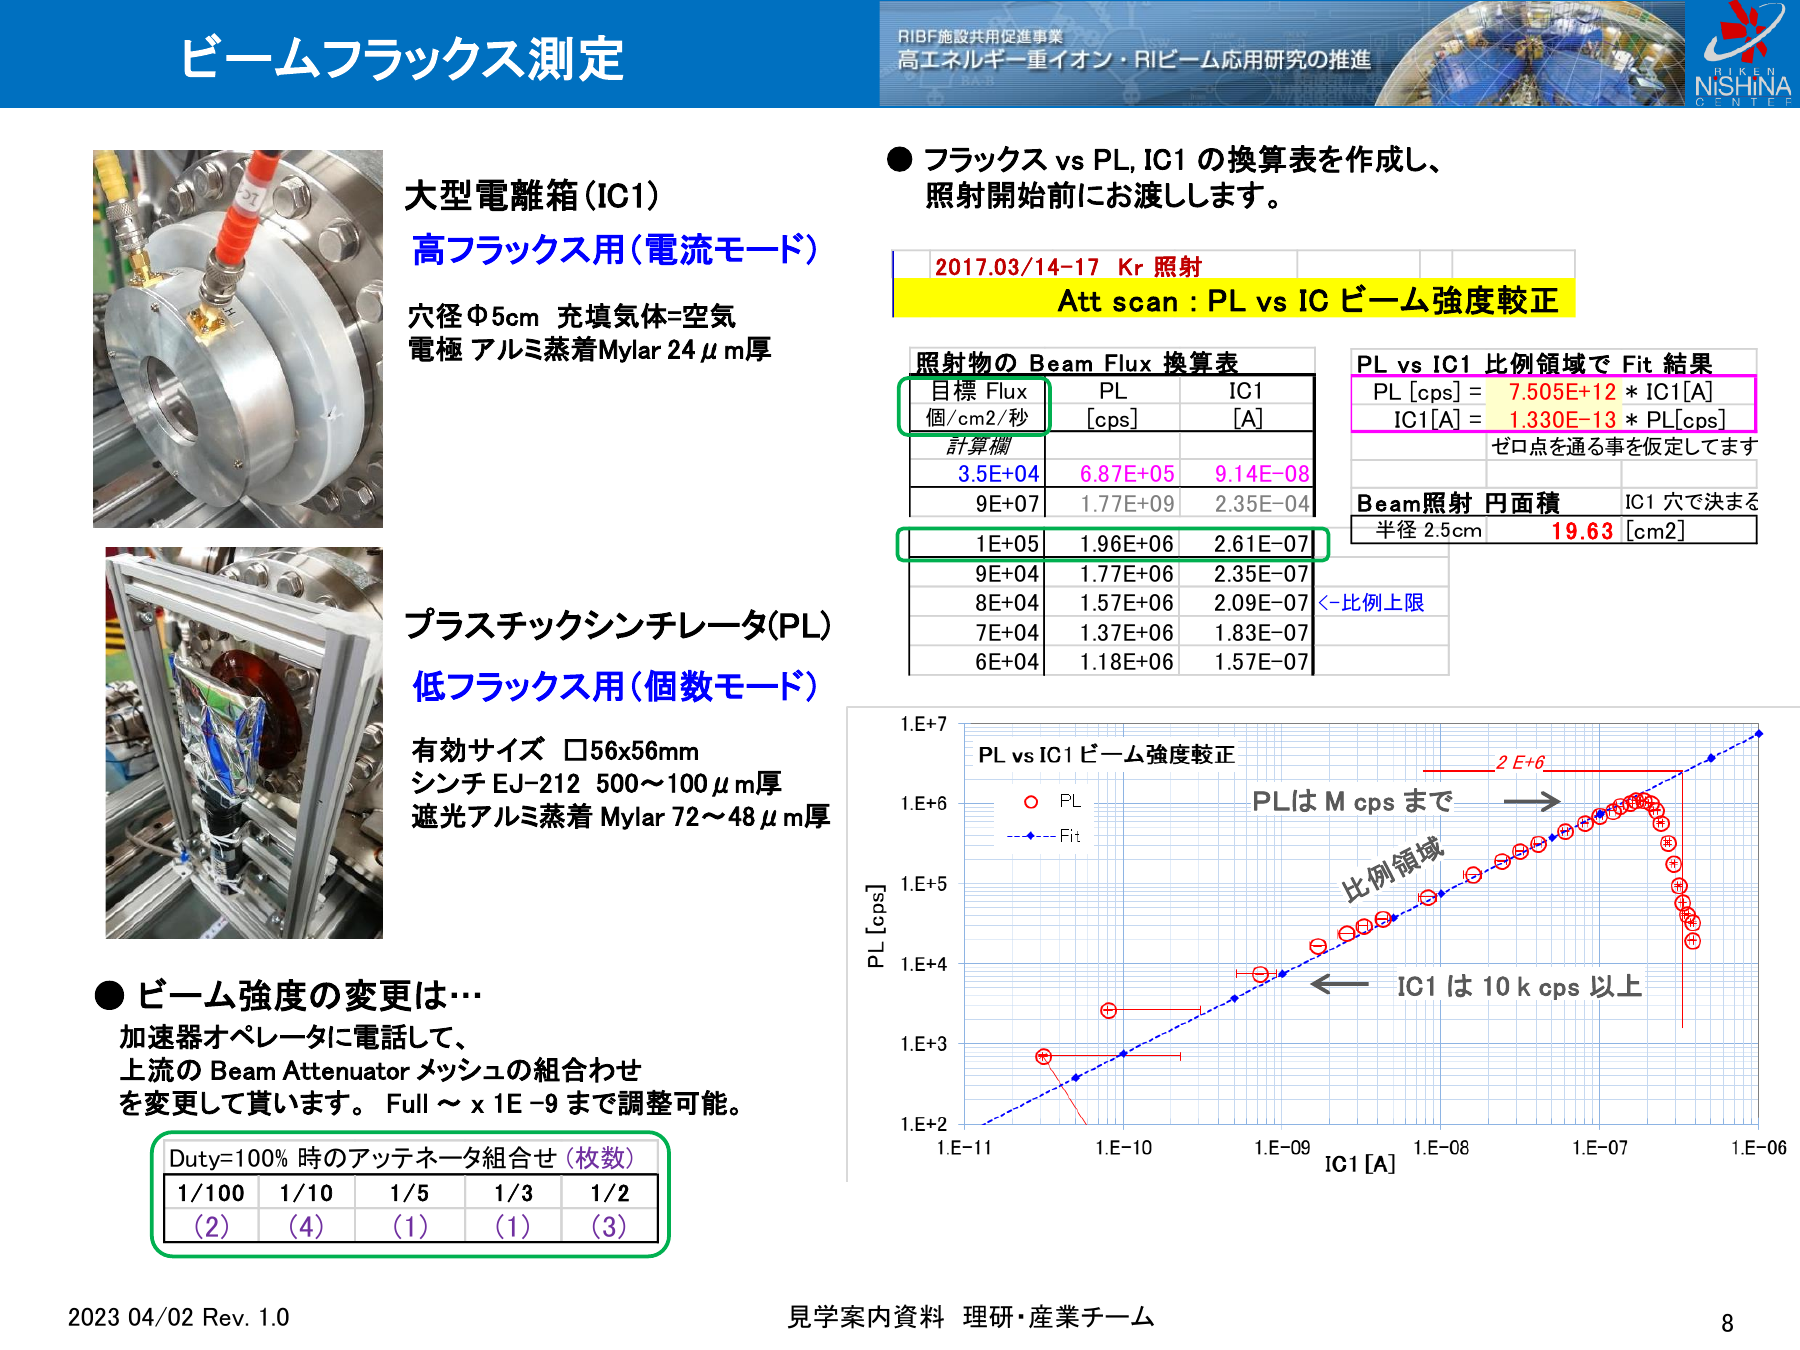
\includegraphics[width=\linewidth]{e5a-att-calibration.png}
\captionof{figure}{Complete page~8 of the E5A visitor guide.\cite{e5a} The lower-left table gives duty factor, mesh counts and adjustment range. The right-hand panel gives the Kr Att scan, PL/IC1 proportional region and area conversion. Mesh station identifiers are not listed, so the page does not assign every mesh to the PIS route.}
\label{fig:e5a-att}
\end{center}

\clearpage
\subsection{Hardware evidence along the AVF/RILAC2--RRC line}
\begin{center}
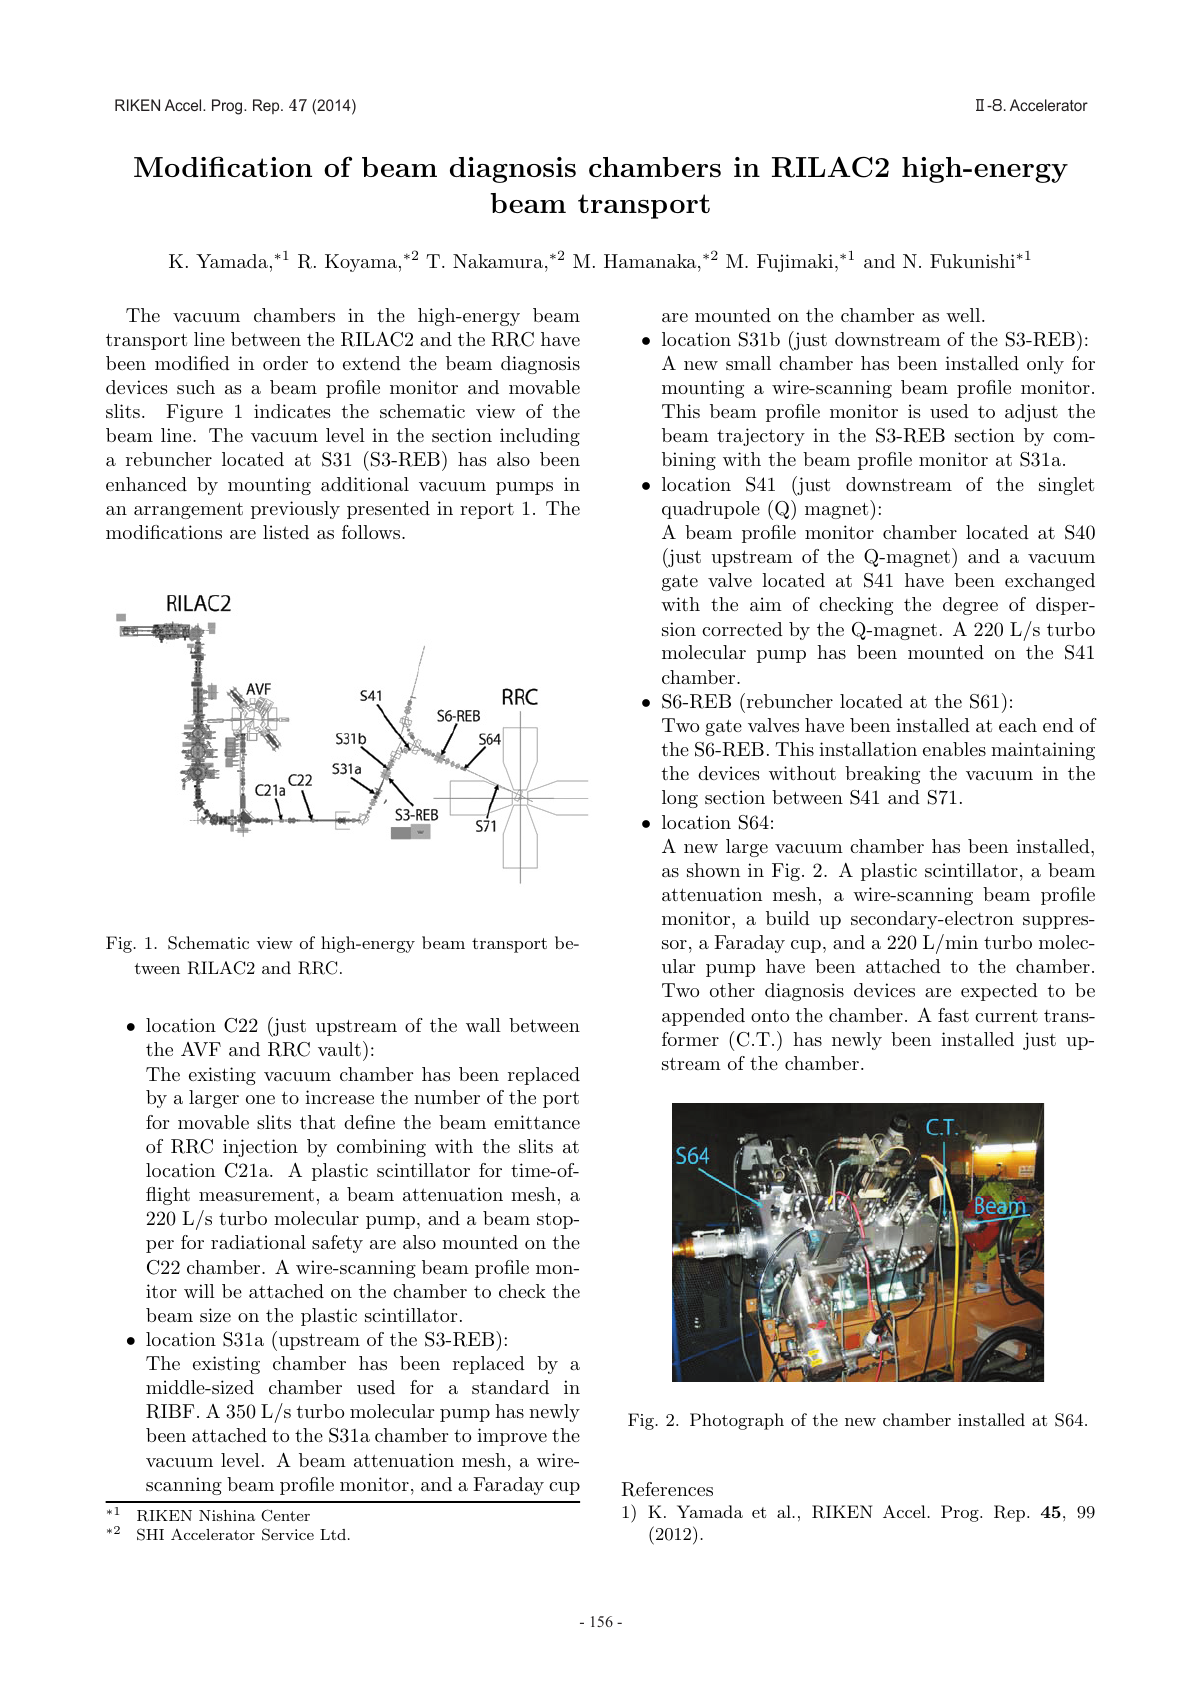
\includegraphics[width=0.85\linewidth]{att-chambers-2014.png}
\captionof{figure}{Yamada et al., 2014 report, printed p.~156.\cite{att-chambers} Original Fig.~1 shows the AVF junction and stations including C22, S31a, S61 and S64. The text identifies three mesh installations; original Fig.~2 shows the S64 diagnostic chamber. This page does not give the five ATT ratios.}
\label{fig:att-location}
\end{center}

\clearpage
\subsection{F3 total rate and BigRIPS stages}
\begin{center}

\includegraphics[width=\linewidth]{f3-limit.png}
\captionof{figure}{F3 total-rate limit. Source: RIKEN, ``Secondary beam intensity expected'', Additional instruction (1), proposal cover-sheet instruction.\cite{bigrips-intensity} It directly specifies $10^7$/s and the Faraday Cup~2 check in LISE++. Orange text is part of the original webpage.}
\label{fig:f3-source}
\end{center}
\begin{center}
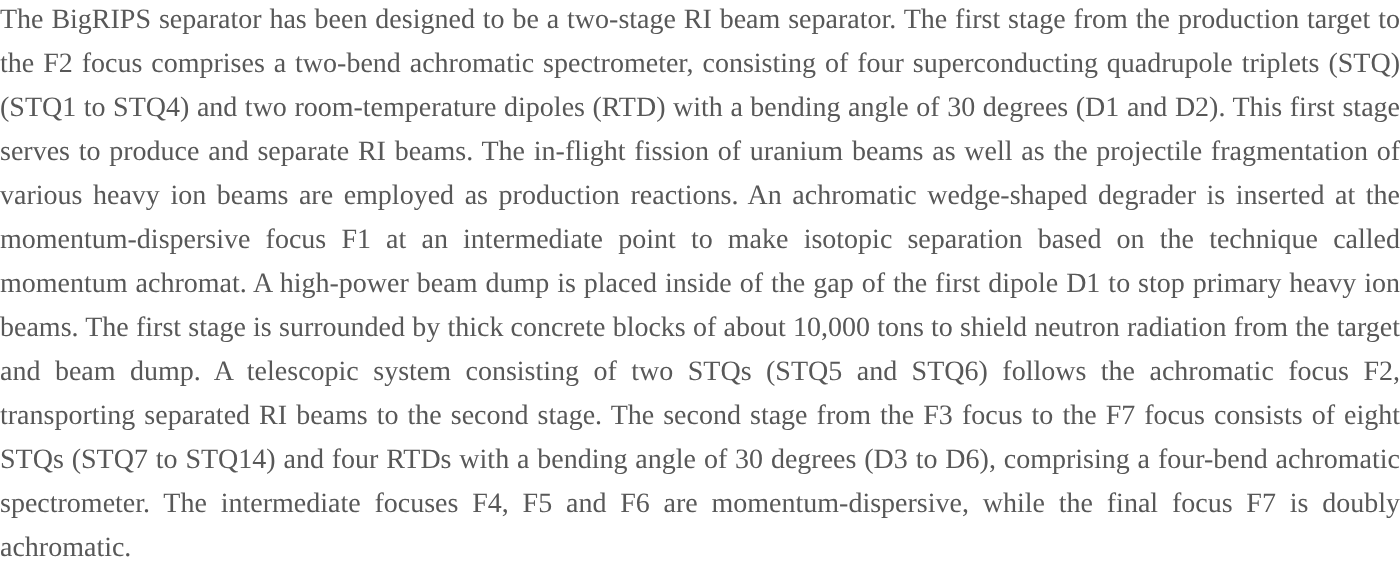
\includegraphics[width=\linewidth]{config-stages.png}
\captionof{figure}{BigRIPS stages, the dispersive F1 focus, and the dump inside D1. Source: opening paragraph of the official configuration page.\cite{bigrips-config} The 8.8-m F2--F3 length is listed separately in the technical table.\cite{bigrips-technical}}
\label{fig:config-source}
\end{center}

\clearpage
\subsection{Installed configurations at F1 and F2}
\begin{center}
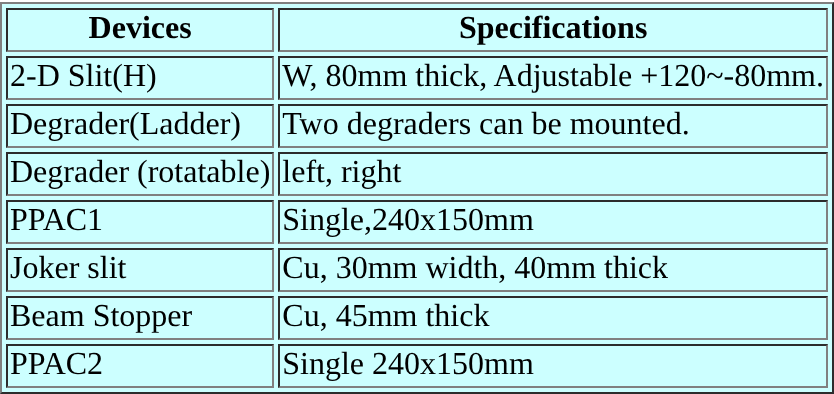
\includegraphics[width=0.90\linewidth]{f1-devices.png}
\par\medskip
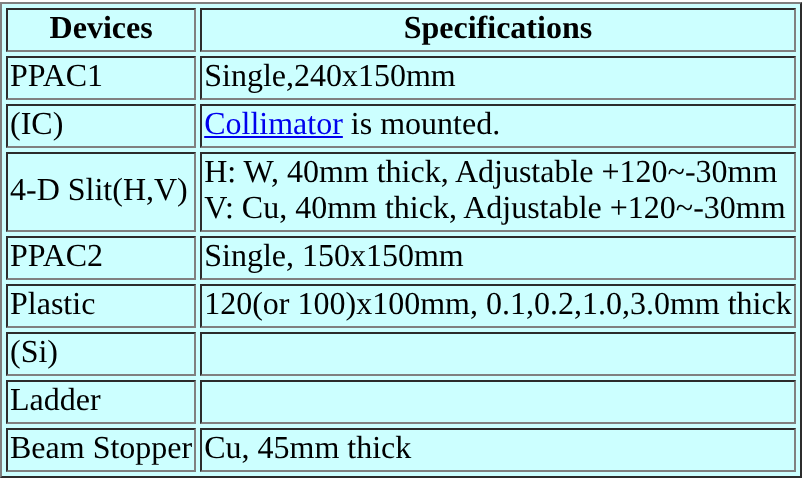
\includegraphics[width=0.98\linewidth]{f2-devices.png}
\captionof{figure}{Top: F1 inventory; bottom: F2 inventory. Source: BigRIPS Team F1/F2 Chamber webpages, dated 27 and 24 August 2018, respectively.\cite{bigrips-focal} F1 lists horizontal slits, a Joker slit, degraders and a stopper. F2 lists 4-D Slit(H,V), a collimator and a 45-mm Cu stopper. These inventories do not specify permissible continuous primary-beam power.}
\label{fig:focal-source}
\end{center}

\clearpage
\subsection{Angular selection at dF2}
\begin{center}
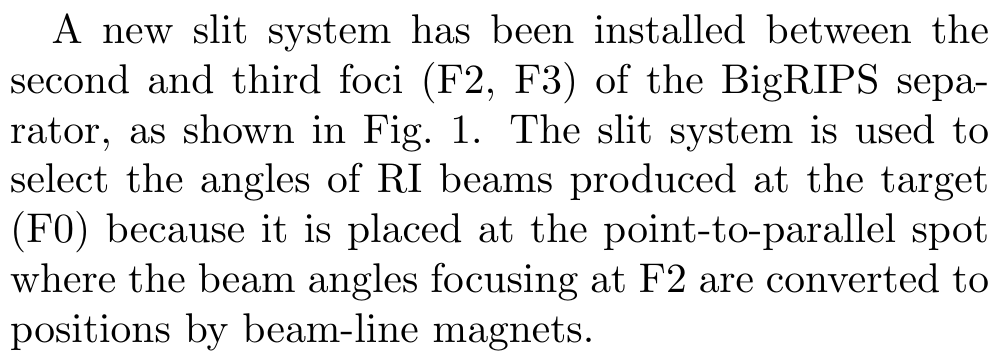
\includegraphics[width=0.85\linewidth]{slit-principle.png}
\par\bigskip
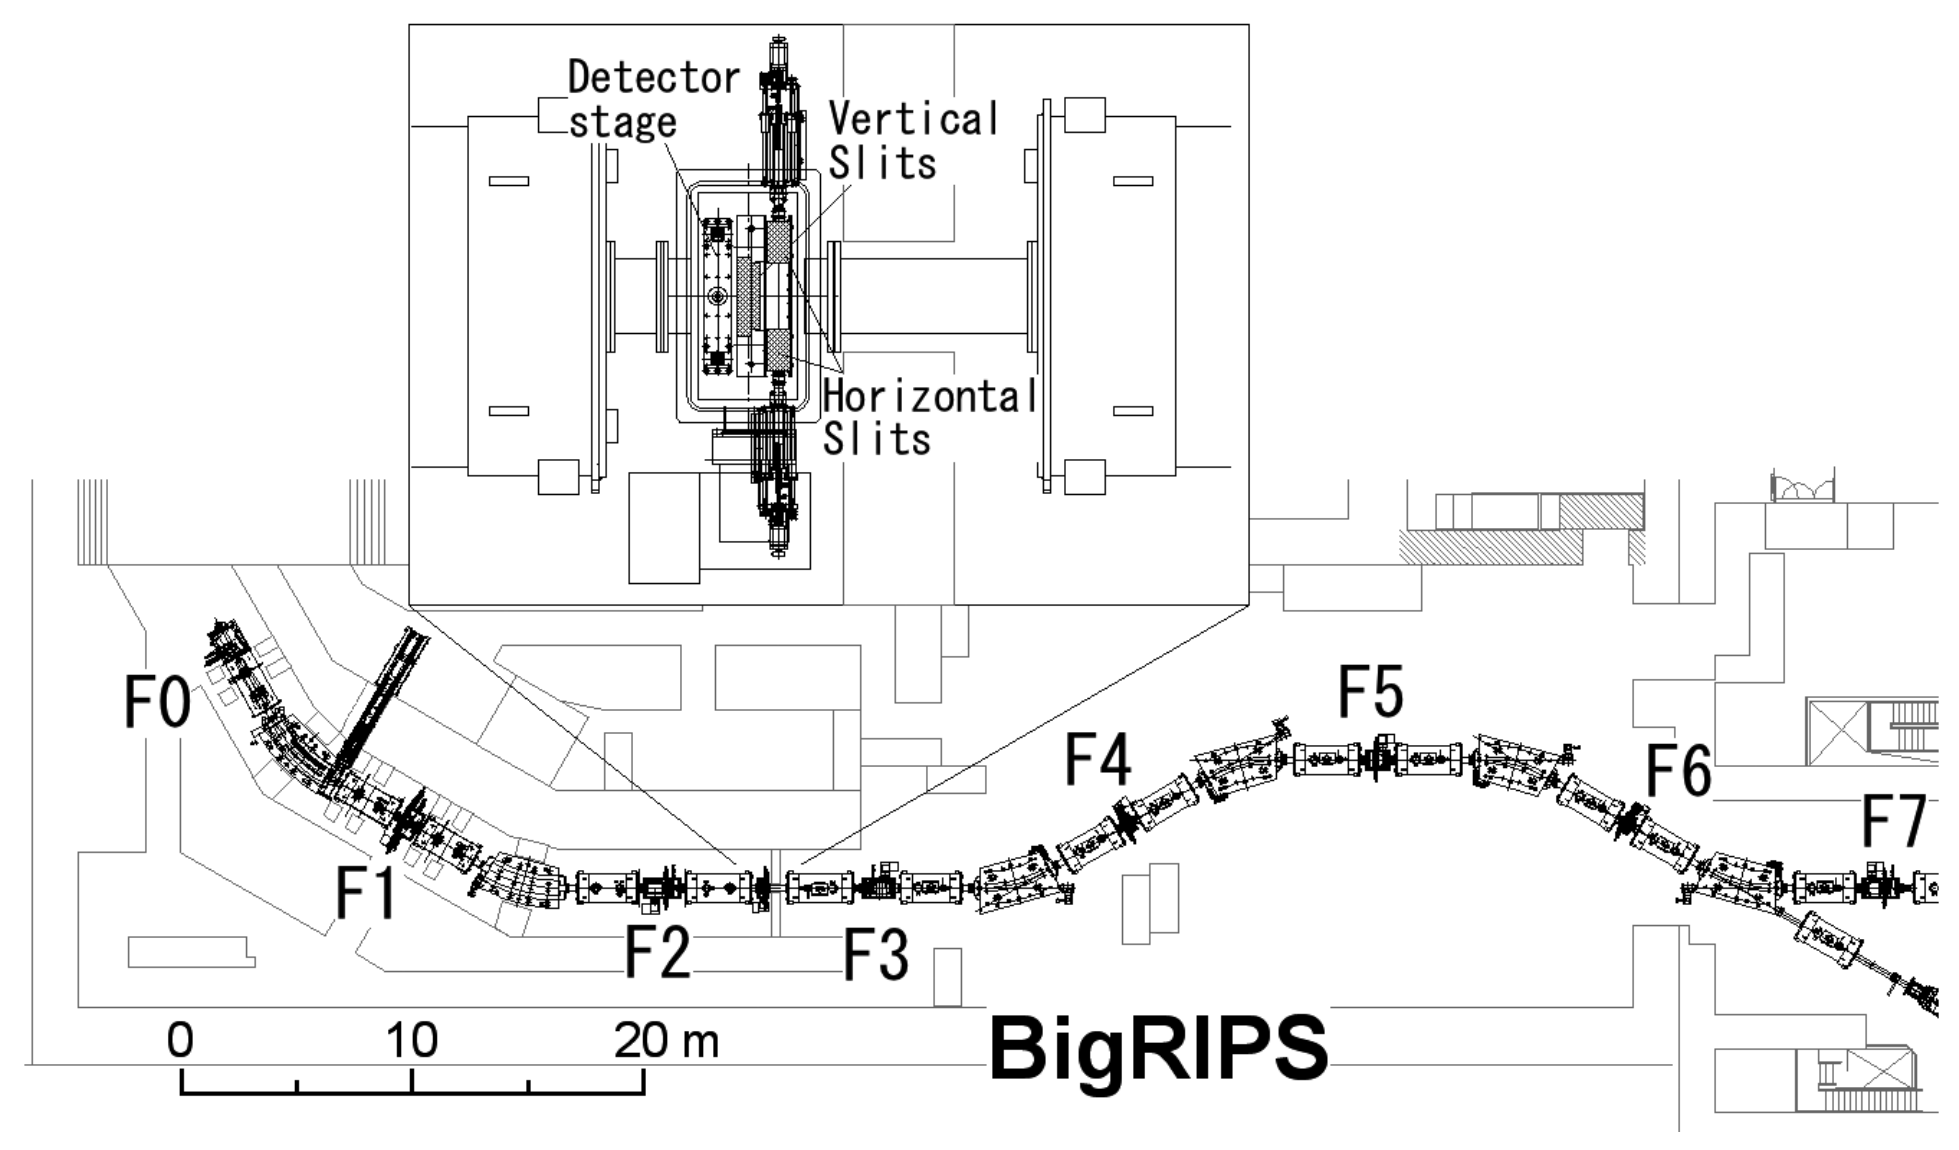
\includegraphics[width=\linewidth]{slit-layout.png}
\captionof{figure}{Top: opening paragraph; bottom: layout from original Fig.~1. Source: Yoshida et al., RIKEN Accel. Prog. Rep.~52 (2019), printed p.~130 / PDF p.~1.\cite{f2-f3-slit} The point-to-parallel optics convert angles at F2 into positions at the slits. The layout locates the horizontal and vertical slits between F2 and F3.}
\label{fig:slit-source}
\end{center}

\clearpage
\subsection{ATT interlock and the SRC exit Faraday cup}
\begin{center}
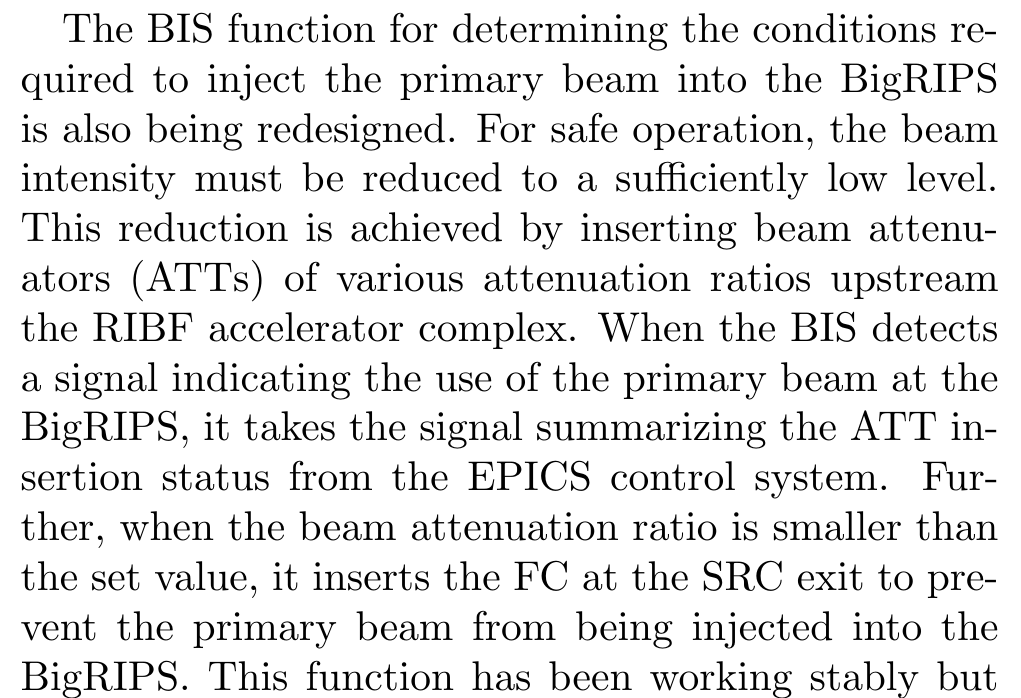
\includegraphics[width=0.85\linewidth]{bis-attenuator.png}
\captionof{figure}{Komiyama et al., RIKEN Accel. Prog. Rep.~58 (2025), final paragraph of the right column on printed p.~98 / PDF p.~1.\cite{bis} Upstream ATT states enter the BIS decision; insufficient attenuation causes insertion of the SRC exit FC to prevent primary-beam delivery to BigRIPS. The paragraph continues on printed p.~99 in the linked source.}
\label{fig:bis-source}
\end{center}
The passage supports the use of upstream attenuation states in the primary-beam injection interlock. It does not give the threshold for this experiment or establish F2/dF2 slits as high-power substitutes for ATTs. The operating conditions therefore remain a matter for the beamline team.
\end{document}
